%  LaTeX support: latex@mdpi.com 
%  For support, please attach all files needed for compiling as well as the log file, and specify your operating system, LaTeX version, and LaTeX editor.

%=================================================================
\documentclass[aerospace,article,submit,moreauthors,dvi2pdf]{Definitions/mdpi} 

% For posting an early version of this manuscript as a preprint, you may use "preprints" as the journal and change "submit" to "accept". The document class line would be, e.g., \documentclass[preprints,article,accept,moreauthors,pdftex]{mdpi}. This is especially recommended for submission to arXiv, where line numbers should be removed before posting. For preprints.org, the editorial staff will make this change immediately prior to posting.

%--------------------
% Class Options:
%--------------------
%----------
% journal
%----------
% Choose between the following MDPI journals:
% acoustics, actuators, addictions, admsci, adolescents, aerospace, agriculture, agriengineering, agronomy, ai, algorithms, allergies, analytica, animals, antibiotics, antibodies, antioxidants, appliedchem, applmech, applmicrobiol, applnano, applsci, arts, asi, atmosphere, atoms, audiolres, automation, axioms, batteries, bdcc, behavsci, beverages, biochem, bioengineering, biologics, biology, biomechanics, biomedicines, biomedinformatics, biomimetics, biomolecules, biophysica, biosensors, biotech, birds, bloods, brainsci, buildings, businesses, cancers, carbon, cardiogenetics, catalysts, cells, ceramics, challenges, chemengineering, chemistry, chemosensors, chemproc, children, civileng, cleantechnol, climate, clinpract, clockssleep, cmd, coatings, colloids, compounds, computation, computers, condensedmatter, conservation, constrmater, cosmetics, crops, cryptography, crystals, curroncol, cyber, dairy, data, dentistry, dermato, dermatopathology, designs, diabetology, diagnostics, digital, disabilities, diseases, diversity, dna, drones, dynamics, earth, ebj, ecologies, econometrics, economies, education, ejihpe, electricity, electrochem, electronicmat, electronics, encyclopedia, endocrines, energies, eng, engproc, entropy, environments, environsciproc, epidemiologia, epigenomes, fermentation, fibers, fire, fishes, fluids, foods, forecasting, forensicsci, forests, fractalfract, fuels, futureinternet, futuretransp, futurepharmacol, futurephys, galaxies, games, gases, gastroent, gastrointestdisord, gels, genealogy, genes, geographies, geohazards, geomatics, geosciences, geotechnics, geriatrics, hazardousmatters, healthcare, hearts, hemato, heritage, highthroughput, histories, horticulturae, humanities, hydrogen, hydrology, hygiene, idr, ijerph, ijfs, ijgi, ijms, ijns, ijtm, ijtpp, immuno, informatics, information, infrastructures, inorganics, insects, instruments, inventions, iot, j, jcdd, jcm, jcp, jcs, jdb, jfb, jfmk, jimaging, jintelligence, jlpea, jmmp, jmp, jmse, jne, jnt, jof, joitmc, jor, journalmedia, jox, jpm, jrfm, jsan, jtaer, jzbg, kidney, land, languages, laws, life, liquids, literature, livers, logistics, lubricants, machines, macromol, magnetism, magnetochemistry, make, marinedrugs, materials, materproc, mathematics, mca, measurements, medicina, medicines, medsci, membranes, metabolites, metals, metrology, micro, microarrays, microbiolres, micromachines, microorganisms, minerals, mining, modelling, molbank, molecules, mps, mti, nanoenergyadv, nanomanufacturing, nanomaterials, ncrna, network, neuroglia, neurolint, neurosci, nitrogen, notspecified, nri, nursrep, nutrients, obesities, oceans, ohbm, onco, oncopathology, optics, oral, organics, osteology, oxygen, parasites, parasitologia, particles, pathogens, pathophysiology, pediatrrep, pharmaceuticals, pharmaceutics, pharmacy, philosophies, photochem, photonics, physchem, physics, physiolsci, plants, plasma, pollutants, polymers, polysaccharides, proceedings, processes, prosthesis, proteomes, psych, psychiatryint, publications, quantumrep, quaternary, qubs, radiation, reactions, recycling, regeneration, religions, remotesensing, reports, reprodmed, resources, risks, robotics, safety, sci, scipharm, sensors, separations, sexes, signals, sinusitis, smartcities, sna, societies, socsci, soilsystems, solids, sports, standards, stats, stresses, surfaces, surgeries, suschem, sustainability, symmetry, systems, taxonomy, technologies, telecom, textiles, thermo, tourismhosp, toxics, toxins, transplantology, traumas, tropicalmed, universe, urbansci, uro, vaccines, vehicles, vetsci, vibration, viruses, vision, water, wevj, women, world 

%---------
% article
%---------
% The default type of manuscript is "article", but can be replaced by: 
% abstract, addendum, article, book, bookreview, briefreport, casereport, comment, commentary, communication, conferenceproceedings, correction, conferencereport, entry, expressionofconcern, extendedabstract, datadescriptor, editorial, essay, erratum, hypothesis, interestingimage, obituary, opinion, projectreport, reply, retraction, review, perspective, protocol, shortnote, studyprotocol, systematicreview, supfile, technicalnote, viewpoint, guidelines, registeredreport, tutorial
% supfile = supplementary materials

%----------
% submit
%----------
% The class option "submit" will be changed to "accept" by the Editorial Office when the paper is accepted. This will only make changes to the frontpage (e.g., the logo of the journal will get visible), the headings, and the copyright information. Also, line numbering will be removed. Journal info and pagination for accepted papers will also be assigned by the Editorial Office.

%------------------
% moreauthors
%------------------
% If there is only one author the class option oneauthor should be used. Otherwise use the class option moreauthors.

%---------
% pdftex
%---------
% The option pdftex is for use with pdfLaTeX. If eps figures are used, remove the option pdftex and use LaTeX and dvi2pdf.

%=================================================================
\graphicspath{{figs/}}
% MDPI internal commands
\firstpage{1} 
\makeatletter 
\setcounter{page}{\@firstpage} 
\makeatother
\pubvolume{1}
\issuenum{1}
\articlenumber{0}
\pubyear{2021}
\copyrightyear{2020}
%\externaleditor{Academic Editor: Firstname Lastname} % For journal Automation, please change Academic Editor to "Communicated by"
\datereceived{} 
\dateaccepted{} 
\datepublished{} 
\hreflink{https://doi.org/} % If needed use \linebreak
%------------------------------------------------------------------
% The following line should be uncommented if the LaTeX file is uploaded to arXiv.org
%\pdfoutput=1

%=================================================================
\usepackage{arydshln}
 \usepackage{multirow}
 \usepackage{siunitx}
 \usepackage{wasysym}
  \usepackage{cases}
% Add packages and commands here. The following packages are loaded in our class file: fontenc, inputenc, calc, indentfirst, fancyhdr, graphicx, epstopdf, lastpage, ifthen, lineno, float, amsmath, setspace, enumitem, mathpazo, booktabs, titlesec, etoolbox, tabto, xcolor, soul, multirow, microtype, tikz, totcount, changepage, paracol, attrib, upgreek, cleveref, amsthm, hyphenat, natbib, hyperref, footmisc, url, geometry, newfloat, caption
%=================================================================
%% Please use the following mathematics environments: Theorem, Lemma, Corollary, Proposition, Characterization, Property, Problem, Example, ExamplesandDefinitions, Hypothesis, Remark, Definition, Notation, Assumption
%% For proofs, please use the proof environment (the amsthm package is loaded by the MDPI class).

%=================================================================
% Full title of the paper (Capitalized)
\Title{A Machine Learning Approach for Global Steering Control Moment Gyroscope Clusters}

% MDPI internal command: Title for citation in the left column
\TitleCitation{A Machine Learning Approach for Global Steering Control Moment Gyroscope Clusters}

% Author Orchid ID: enter ID or remove command
\newcommand{\orcidauthorA}{0000-0003-3114-3330} % Add \orcidA{} behind the author's name
%\newcommand{\orcidauthorB}{0000-0000-0000-000X} % Add \orcidB{} behind the author's name

% Authors, for the paper (add full first names)
\Author{Charalampos Papakonstantinou $^{1,}$*\orcidA{}, Ioannis Daramouskas $^{1}$, Vaios Lappas $^{2}$, Vassilis C. Moulianitis $^{3}$ and {Vassilis Kostopoulos} $^{4}$}

% MDPI internal command: Authors, for metadata in PDF
\AuthorNames{Charalampos Papakonstantinou, Ioannis Daramouskas, Vaios Lappas, Vassilis C. Moulianitis and Vassilis Kostopoulos}

% MDPI internal command: Authors, for citation in the left column
\AuthorCitation{Papakonstantinou, C.; Daramouskas, I.; Lappas, V.; Moulianitis, C. V.; Kostopoulos, V.}
% If this is a Chicago style journal: Lastname, Firstname, Firstname Lastname, and Firstname Lastname.

% Affiliations / Addresses (Add [1] after \address if there is only one affiliation.)
\address{%
$^{1}$ \quad Department of Mechanical Engineering and Aeronautics, University of Patras, 26504 Patras, Greece; daramousk@ceid.upatras.gr\\

$^{2}$ \quad Department of Aerospace Science and Technology, National Kapodistrian University of Athens, \mbox{10679 Athens, Greece}; vlappas@upatras.gr\\
$^{3}$ \quad Department of Product and Systems Design Engineering, University of the Aegean, 84100 Syros, Greece; moulianitis@syros.aegean.gr\\
$^{4}$ \quad Applied Mechanics and Vibrations Laboratory, Department of Mechanical Engineering and Aeronautics, University of Patras, 26504 Patras, Greece; kostopoulos@upatras.gr\\
}

% Contact information of the corresponding author
\corres{Correspondence: c\_papakonstantinou@upnet.gr;
Tel.: +30-698-912-4655;+0000-0003-3114-3330}


% The commands \thirdnote{} till \eighthnote{} are available for further notes

%\simplesumm{} % Simple summary

%\conference{} % An extended version of a conference paper

% Abstract (Do not insert blank lines, i.e. \\) 
\abstract{This paper addresses the problem of singularity avoidance for a 4-Control Moment Gyroscope (CMG) pyramid cluster, as used for the attitude control of a satellite using machine learning (ML) techniques. A data-set, generated using a heuristic algorithm, relates the initial gimbal configuration and the desired manoeuvre - inputs - to a number of null space motions the gimbals have to execute - output. Two ML techniques - Deep Neural Network (DNN) and Random Forest Classifier (RFC) - are utilized to predict the required null motion for trajectories that are not included in the training set. The principal advantage of this approach is the exploitation of global information gathered from the whole manoeuvre compared to conventional steering laws that consider only some local information, near the current gimbal configuration for optimization. The data-set generation and the predictions of the ML systems can be made offline, so no further calculations are needed on board, providing the possibility to inspect the way the system responds to any commanded manoeuvre before its execution. The RFC technique demonstrates enhanced accuracy for the test data compared to the DNN, validating that it is possible to predict correctly the null motion even for manoeuvres that are not included in the training data.}

% Keywords
\keyword{Spacecraft attitude control, control moment gyroscope cluster, pyramid configuration, global steering, machine learning, deep neural network, random forest classifier} 

% The fields PACS, MSC, and JEL may be left empty or commented out if not applicable
%\PACS{J0101}
%\MSC{}
%\JEL{}

%%%%%%%%%%%%%%%%%%%%%%%%%%%%%%%%%%%%%%%%%%
% Only for the journal Diversity
%\LSID{\url{http://}}

%%%%%%%%%%%%%%%%%%%%%%%%%%%%%%%%%%%%%%%%%%
% Only for the journal Applied Sciences:
%\featuredapplication{Authors are encouraged to provide a concise description of the specific application or a potential application of the work. This section is not mandatory.}
%%%%%%%%%%%%%%%%%%%%%%%%%%%%%%%%%%%%%%%%%%

%%%%%%%%%%%%%%%%%%%%%%%%%%%%%%%%%%%%%%%%%%
% Only for the journal Data:
%\dataset{DOI number or link to the deposited data set in cases where the data set is published or set to be published separately. If the data set is submitted and will be published as a supplement to this paper in the journal Data, this field will be filled by the editors of the journal. In this case, please make sure to submit the data set as a supplement when entering your manuscript into our manuscript editorial system.}

%\datasetlicense{license under which the data set is made available (CC0, CC-BY, CC-BY-SA, CC-BY-NC, etc.)}

%%%%%%%%%%%%%%%%%%%%%%%%%%%%%%%%%%%%%%%%%%
% Only for the journal Toxins
%\keycontribution{The breakthroughs or highlights of the manuscript. Authors can write one or two sentences to describe the most important part of the paper.}

%%%%%%%%%%%%%%%%%%%%%%%%%%%%%%%%%%%%%%%%%%
% Only for the journal Encyclopedia
%\encyclopediadef{Instead of the abstract}
%\entrylink{The Link to this entry published on the encyclopedia platform.}
%%%%%%%%%%%%%%%%%%%%%%%%%%%%%%%%%%%%%%%%%%

\begin{document}
%%%%%%%%%%%%%%%%%%%%%%%%%%%%%%%%%%%%%%%%%%
% \setcounter{section}{-1} %% Remove this when starting to work on the template.

\section{Introduction}

Control Moment Gyroscopes (CMGs) are widely used in spacecraft control for manoeuvring and they have been successfully employed for a wide range of space missions \cite{futuremissions,defendini,wie2008space}. Since they are momentum-exchange actuators, the shape and the size of the momentum envelope depends on their configuration. The size of the envelope is proportional to the maximum available torque that can be generated in a certain directions. From all the possible configurations, the conceptual pyramid configuration is commonly studied in the literature due to the nearly 3-axis symmetric and spherical momentum envelope it produces \cite{SMCS}. Despite the extreme torque magnification property and the rapid response, the singularity problem poses a barrier to make CMGs popular in attitude control\cite{Bang},\cite{Lian}. In general, singular states are divided in two main categories. If a singular state can be escaped by null motion, it is classified as passable or hyperbolic \cite{Margulies}, otherwise, the singularity is  referred as elliptic. In both cases, the manipulability index can be used as a performance measure to indicate the approach to singularity as proposed in \cite{yoshikawa}. An extensive study in singularities topology has been made in \cite{Hirohisa2014,Rapid_Guo,Kurokawa1994}. Dealing with singular states is commonly classified  in two different categories: the singularity avoidance and the singularity escape logics \cite{HybridSteering}. The steering logics that avoid a singular state without creating torque error, being usually more precise, are included in the first category whereas the steering logics that induce torque error to escape a singularity, commonly trying to minimize it, belong to the second one. Both approaches make use of some local information in the vicinity of the current gimbal configuration \cite{bongwie2005},\cite{bongwie2001}. 

Path planing techniques that take into consideration the whole manoeuvre are usually focusing in choosing the initial gimbal configuration that optimizes the performance of the system during the trajectory \cite{vadali_preferred}. A global steering path planing approach is discussed in \cite{paradiso},\cite{paradiso2} where an A* search algorithm is used to steer the gimbals of a CMG cluster in the null space. An enhanced global steering approach is also presented in \cite{Papakonstantinou}, that does not use a node visit histogram and offers the possibility for near-real time implementation. Such approaches are capable of dealing with singularities before encountering them but a new optimization problem has to be solved for every manoeuvre commanded.

The advances in computer science and Machine Learning (ML) are establishing a new era for a variety of science fields even though models of artificial neural networks have been used since about the 1950s \cite{rosenblatt}. The developed algorithms are employed in pattern recognition, object detection and numerous aerospace-related applications \cite{pritmark,Cornejo,Ferreira}.  The availability of a great amount of information and data is encouraging the substitution of the heuristic approaches, that are widely used so far, by machine learning techniques. Combining data-sets with the computational efficiency of modern computers, it is possible to create a system able to learn and come into conclusions as well as a humans do. However, in the field of CMGs no extended research has been conducted from the perspective of ML. An adaptive control approach using neural networks for spacecraft systems with uncertainty under external disturbances is proposed in \cite{Leeghim} whilst an estimation of gimbal angles through a similar network is discussed in \cite{Zhong}. However, no research has been done in relating the null space motion with the initial gimbal configuration and the desired manoeuvre through a data-set. 

In this paper, a method of improving the performance of a spacecraft employed with CMGs by investigating an optimal path in the gimbals' null space is presented. It takes into consideration the whole desired/commanded manoeuvre (global search), in contrast to the most conventional gradient methods that exploit some information only in the region near the low performance configurations. Two different ML techniques - Deep Neural Network (DNN) and Random Forest Classifier (RFC) - are implemented to deal with the global steering problem, without the need of creating and searching a new graph every time a new manoeuvre has to be executed. A data-set that relates the initial gimbal angles and the commanded quaternion with the desired null motion is developed using a heuristic algorithm. The desired null motion is selected to maximize a singularity related Objective Function (OF) and the data-set is used to train the two ML systems. The OF is defined as the minimum value of the manipulability index across the manoeuvre. A part of the data-set, i.e the test data-set, is used to evaluate the ability of the ML systems to efficiently predict and generalize the results for unknown input data. The method proposed in this paper allows the null motion path to be derived offline before commanding the satellite to execute the manoeuvre, and as a result it can be used for inspection. Moreover, a comparison is held among the ML techniques and the Null Space Projection (NSP). The results indicate that for the same manoeuvre, the execution time required is significantly lower in the case of DNNs and RFC, compared to the NSP and the minimum manipulability value is higher when RFC is used. The method proposed combines high scalability, as long as the dynamic model of the satellite can be calculated, with reduced complexity once the ML model has been trained.

The paper is structured as follows. In sections II and III, the rigid spacecraft equations of motion and the control law used are described. Section IV and V present the data derivation and simulation results of DNN and RFC compared to the NSP. Finally, the ML systems and the results are briefly summarized in the conclusion section.
 
\section{Mathematical Modeling}
The equation of motion of a rigid spacecraft is described by:

\begin{equation}
\dot{\boldsymbol{\omega}}=\textbf{J}^{-1}(-\boldsymbol{\omega}\times(\textbf{J}\boldsymbol{\omega})-\dot{\textbf{h}}-\boldsymbol{\omega}\times \textbf{h} + \textbf{T}_{ex})
\label{eq:dyn_eq}
\end{equation}
where $\textbf{T}_{ex} \in { \Re  }^{ 3\times1}$ is the vector that represents the external torques applied to the spacecraft and $\boldsymbol{\omega} \in {\Re}^{3\times1}$ denotes the angular velocity of the spacecraft with respect to the body frame. The control torque, $\textbf{T}_c  \in {\Re}^{3\times1}$ can be selected as \cite{lappasthesis}:

\begin{equation}
\dot { \textbf{h} } +\boldsymbol{\omega}\times \textbf{h}=-\textbf{ T }_c
\label{eq:control}
\end{equation}
where $ \textbf{h}\in\Re^{3\times1}$ is the angular momentum of the CMG cluster:

\begin{equation}
\textbf{h}=h_0
\begin{bmatrix}
-c\beta s\delta_1-c\delta_2+c\beta s\delta_3+c\delta_4 \\
c\delta_1 -c\beta s\delta_2 -c\delta_3 +c\beta s\delta_4 \\
s\beta s\delta_1+s\beta s\delta_2+s\beta s\delta_3+s\beta s\delta_4
\end{bmatrix}  
\end{equation}
and $s$, $c$ are the abbreviations for $\sin$ and $\cos$ respectively.  The parameter $\beta$ denotes the skew angle of the 4-CMG cluster in pyramid configuration and it is chosen properly in order the momentum envelope to be nearly tree-axis symmetric and spherical. $h_0$ is the magnitude of the momentum of each flywheel which can be considered equal to one.
In general, the momentum derived from the CMG cluster is a function of the gimbal angles $\boldsymbol{\delta}=[\delta_1, \delta_2,\delta_3, \delta_4]^T\in\Re^{4\times1}$ for a spacecraft employed with 4 CMGs. Assuming that the control torque is known, the relation between the total CMG momentum rate and the gimbal angles rates  can be derived by the equation:

\begin{equation}
   \dot{ \textbf{h}}=\textbf{A}(\boldsymbol{\delta})\dot{\boldsymbol{\delta}}
\end{equation}
where $\textbf{A}(\boldsymbol{\delta})\in\Re^{3\times4} $ is the Jacobian matrix of the system and it is a function of the gimbal angles and the skew angle. For the 4-CMG cluster the Jacobian matrix is calculated by:

\begin{equation}
\textbf{A}(\boldsymbol{\delta})=
\begin{bmatrix}
-c\beta c\delta_{1} & s\delta_{2} & c\beta c\delta_{3} & -s\delta_{4}\\
-s\delta_{1} & -c\beta c\delta_{2} & s\delta_{3} & c\beta c\delta_{4}\\
s\beta c\delta_{1} & s\beta c\delta_{2} & s\beta c\delta_{3} & s\beta c\delta_{4}
\end{bmatrix}
\end{equation}
and the gimbal angle rate vector $\boldsymbol{\dot{\delta}}\in\Re^{4\times1}$ is given by:

\begin{equation}
\label{eq:inverse}
   \dot{\boldsymbol{\delta}}=\textbf{A}^\#(\boldsymbol{\delta}) \dot{ \textbf{h}}
\end{equation}
Since the Jacobian matrix is not rectangular, several definitions have been discussed for the inverse of the Jacobian matrix $\textbf{A}^\#(\boldsymbol{\delta})$ \cite{bongwie2001}.

The satellite's kinematics equations of motion expressed in quaternion form are given by:

\begin{equation}
\dot{\textbf{q}}=\frac{1}{2}\textbf{q}\odot\boldsymbol{\omega}_q
\label{eq:quaternion_dot}
\end{equation}
where $\odot$ denotes the quaternion multiplication and $\textbf{q}=[q_0, q_1, q_2, q_3]^T\in\Re^{4\times1}$ represents the attitude quaternion. $\boldsymbol{\omega}_q=[0,\boldsymbol{\omega}^T]^T\in\Re^{4\times1}$ is the angular velocity $\boldsymbol{\omega}$ of the spacecraft given in quaternion form. For two quaternions $\textbf{r}=[r_0,r_1,r_2,r_3]^T\in\Re^{4\times1}$ and $\textbf{p}=[p_0,p_1,p_2,p_3]^T\in\Re^{4\times1}$ the quaternion multiplication is defined as:

\begin{equation}
\textbf{r} \odot \textbf{p} =
\begin{bmatrix}
p_0r_0 - p_1r_1 - p_2r_2 - p_3r_3\\
 p_0r_1 + p_1r_0 - p_2r_3 + p_3r_2\\
 p_0r_2 + p_2r_0 + p_1r_3 - p_3r_1\\
 p_0r_3 - p_1r_2 + p_2r_1 + p_3r_0\\
\end{bmatrix}
\end{equation}
For the implementation of the attitude control, the control torque $\textbf{T}_c \in\Re^{3\times1}$ applied on the satellite's body is a function of the vector part of the error quaternion $\textbf{q}_{err}$ and $\boldsymbol{\omega}$ as described by the following equation:

\begin{equation}
\textbf{T}_c=-(K_p\textbf{q}_{err}^v
+K_i\int\textbf{q}_{err}^vdt+K_{\omega}\boldsymbol{\omega})
\end{equation}
The error quaternion between the current attitude quaternion and the commanded quaternion $\textbf{q}^c$ is : 

\begin{equation}
\textbf{q}_{err}=
\begin{bmatrix}
q_{err}^s\\
\textbf{q}_{err}^v
\end{bmatrix}={\textbf{q}^{c}}^{*}\odot\textbf{q}
\end{equation}
where $q_{err}^s$ and $\textbf{q}_{err}^v=[q_{err}^{roll}, q_{err}^{pitch}, q_{err}^{yaw}]^T \in\Re^{3\times1}$ are the scalar and the vector part respectively and ${\textbf{q}^{c}}^{*}$ expresses the conjugate quaternion of $\textbf{q}^c=[q^{c}_0, q^{c}_1, q^{c}_2, q^{c}_3]^T\in\Re^{4\times1}$. The normalization of the quaternions is required before evaluating the $\textbf{q}_{err}$. The "3-2-1" sequence is used to convert the quaternion error to the corresponding Euler angles error.

Since the simulation describes a discrete time system, it is required to integrate the quaternion rate $\dot{\textbf{q}}$ at the $i^{th}$ iteration as given by Equation~(\ref{eq:quaternion_dot}) using the equation:

\begin{equation}
\textbf{q}_i=\textbf{q}_{i-1}\odot[\cos(||\boldsymbol{\omega}||\frac{dt}{2}), \frac{\boldsymbol{\omega}}{||\boldsymbol{\omega}||}\sin(||\boldsymbol{\omega}||\frac{dt}{2})]^T
\end{equation}
where $dt$ is the time-step between two consecutive iterations.
The CMG gimbal angle rates become saturated when they exceed the specific threshold $\dot{{\delta}}_{th}$, using the following formula:

\begin{equation}
\label{eq:saturation}
\dot{\boldsymbol{\delta}}_{sat}=\dot{\boldsymbol{\delta}}\hspace{0.1cm}\frac{\dot{{\delta}}_{th}}{\max(|\dot{\delta}_1|,|\dot{\delta}_2|,|\dot{\delta}_3|,|\dot{\delta}_4|)}
\end{equation}
It is preferred to saturate the gimbal angle rates using Equation~(\ref{eq:saturation}) than applying a boundary value to every gimbal angle rate that exceeds the required threshold since the characteristics of the motion are conserved. 
The Moore-Penrose steering law is used, given by:

\begin{equation}
\textbf{A}^\#=\textbf{A}^T(\textbf{A}\textbf{A}^T)^{-1}
\label{eq:SR_inverse}
\end{equation}
The null motion term is added in Equation~(\ref{eq:inverse}) and is composed of the term $k_i$ and the null gimbal rates $\dot{\boldsymbol{\delta}}_{Null}\in\Re^{4\times1}$ as

\begin{equation}
\label{eq:nullk}
   \dot{\boldsymbol{\delta}}=\textbf{A}^T(\textbf{A}\textbf{A}^T)^{-1} \dot{ \textbf{h}} + 4k_i \dot{\boldsymbol{\delta}}_{Null}
\end{equation}
where

\begin{equation}
\label{eq:nulldelta}
 \dot{\boldsymbol{\delta}}_{Null}=
\begin{bmatrix}
|c_2 \quad c_3 \quad c_4|\\ 
-|c_2 \quad c_3 \quad c_4|\\
|c_2 \quad c_3  \quad c_4|\\
-|c_2  \quad c_3 \quad c_4|
\end{bmatrix}
\end{equation}
and $\textbf{c}_n\in \Re^{3\times1}$represents the output torque of the $n^{th}$ CMG of the cluster, i.e. the $n^{th}$ column of $\textbf{A}$. Let the value of $k_i$ change in each time-step resulting in a different null motion.
 
 
 \section{Data Derivation}

An optimization problem is discussed in this section in order to create the data-set that relates the initial gimbal angles and the commanded quaternion to the null space motion. The desired manoeuvre is divided in $D$ discrete steps and the $k_i$, ($i=1,..,D$) value is determined for the $i$ corresponding step. There are three different values of $k_i$:  $-k_{max}, 0$ and $ +k_{max}$ where $k_{max}$ is a constant value which represents the maximum null motion that can be added to the system in each time-step.
The optimization problem is expressed as:

\begin{equation}
\begin{aligned}
\underset{\textbf{L}}{\text{maximize}} \quad
 \underset{t=1,..,s}{\text{min}}(w_t) \\
\end{aligned}
\label{eq:optimizationproblem}
\end{equation}
where $\textbf{L}=[k_1, k_2, ... , k_D]$, $s$ is the manoeuvre duration and $w_t$ is the manipulability index at time $t$ determined by:

\begin{equation}
w_t=\sqrt{\text{det}(\boldsymbol{A}_t \boldsymbol{A}_t^{\mathrm{T}})}
\label{eq:manipul}
\end{equation}
Since the Jacobian matrix is a function of the gimbal angles that change over time, it can be also considered as a function of time for representation purposes.
A heuristic algorithm is implemented that optimizes the OF of Equation~(\ref{eq:optimizationproblem}) value subject to the $\textbf{L}$ set. The manipulability index is selected because it is a metric of distance from a singularity since it equals to the product of the Jacobian singular values. The OF is related to the minimum value of the manipulability index in order to improve the worst performance configuration through the manoeuvre. This algorithm is based on a tree structure in which each branch corresponds to a different $k_i$ value. As long as the value of the OF remains higher than the best so-far OF value, the tree continues to expand the same branch. Otherwise, the expansion is terminated and the exploration begins in the next branch.  

%  Although, the OF can be expanded to include more terms like the mean value of a performance index and the time the gimbal rates exceed a specific threshold.


In order to generate the desired data-set, multiple initial gimbal angles vectors and commanded quaternion vectors are used. When these inputs are selected randomly, the derived data-set can not be used due to the high standard deviation of the outputs and the amount of outliers existed. Instead, it is preferable to divide the initial gimbal angles into different families. The Binet-Cauchy theorem as implemented for singularity analysis in \cite{bongwie2004} relates the square of $w$ to the sum of the Jacobian minors as

\begin{equation}
w=\mathrm{det}(\boldsymbol{A} \boldsymbol{A}^{\mathrm{T}})=\sum_{n=1}^{4} M_{n}^{2}=0
\end{equation}
where $M_n=\mathrm{det}(\textbf{A}_n), n=1,2...4$ and $\textbf{A}_n$ is the matrix $\textbf{A}$ with the $n^{th}$ column removed. 
The order 3 Jacobian minors $M_n$ are calculated by

\begin{equation}
\begin{matrix}
M_{1}=s \beta[( s \delta_{2} s \delta_{3} c \delta_{4}+c \delta_{2} s \delta_{3} s \delta_{4}) \\
+c \beta(c \delta_{2} c \delta_{3} s \delta_{4}-s \delta_{2} c \delta_{3} c \delta_{4}) +\\
+2 c ^{2} \beta c \delta_{2} c \delta_{3} c \delta_{4}]
\end{matrix}
\label{eq:M1_functions}
\end{equation}
\begin{equation}
\begin{matrix}
M_{2}= s \beta[(s \delta_{3} s \delta_{4} c \delta_{1}+c \delta_{3} s \delta_{4} s \delta_{1})+\\
+c \beta (c \delta_{3} c \delta_{4} s \delta_{1}-s \delta_{3} c \delta_{4} c \delta_{1}) +\\
+2 c ^{2} \beta c \delta_{3} c \delta_{4} c \delta_{1}]
\end{matrix}
\label{eq:M2_functions}
\end{equation}
\begin{equation}
\begin{matrix}
M_{3}=s \beta[(s \delta_{4} s \delta_{1} c \delta_{2}+c \delta_{4} s \delta_{1} s \delta_{2})+\\
+c \beta(c \delta_{4} c \delta_{1} s \delta_{2}-s \delta_{4} c \delta_{1} c \delta_{2}) +\\
+2 c ^{2} \beta c \delta_{4} c \delta_{1} c \delta_{2}]
\end{matrix}
\label{eq:M3_functions}
\end{equation}
\begin{equation}
\begin{matrix}
M_{4}= s \beta[(s \delta_{1} s \delta_{2} c \delta_{3}+c \delta_{1} s \delta_{2} s \delta_{3})+\\
+c \beta(c \delta_{1} c \delta_{2} s \delta_{3}-s \delta_{1} c \delta_{2} c \delta_{3})+ \\
+2 c ^{2} \beta c \delta_{1} c \delta_{2} c \delta_{3}]
\end{matrix}
\label{eq:M4_functions}
\end{equation}

Following this definition, the gimbal angles are classified in families by the sign combinations of the Jacobian minors. That means that every time the a minor changes sign there is a family change. In total, there are $2^4=16$ possible minor sign combinations each one corresponding to one family. The sign of $s\beta$ is the same in all Jacobian minors so the first term in Equations.~(\ref{eq:M1_functions}) - (\ref{eq:M4_functions}) can be ignored. In this paper, the families with respect to the minors sign are presented in Table~\ref{tab:Families}

\begin{specialtable}[hbt!]
\caption{\label{tab:Families} Families}
\begin{tabular}{lcccc}
\toprule
\textbf{Family No.}&$M_1$&$M_2$&$M_3$&$M_4$\\
\midrule
Family 0&+ & + & + & +  \\
Family 1&+ & + & + & -  \\
Family 2&+ & + & - & -  \\
Family 3&+ & + & - & +  \\
Family 4&+ & - & - & +  \\
Family 5&+ & - & - & -  \\
Family 6&+ & - & + & -  \\
Family 7&+ & - & + & +  \\
Family 8&- & - & + & +  \\
Family 9&- & - & + & -  \\
Family 10&- & - & - & -  \\
Family 11&- & - & - & +  \\
Family 12&- & + & - & +  \\
Family 13&- & + & - & -  \\
Family 14&- & + & + & -  \\
Family 15&- & + & + & + \\
\bottomrule
\end{tabular}
\end{specialtable}

To achieve a null motion per simulation time-step $dt=0.01$, for a 20 s simulation, a length of $D=2000$ is required. Such a length is not practical for optimization and  near real time applications in terms of execution time and numerical computations. 
To select a proper depth value, 26 different initial gimbal angles in the range of $[-\pi/2 , \pi/2]$ and 60 different commanded quaternions that belong in the two first families are selected and the OF value is calculated for each combination of them.
It is observed that increasing the depth further than 8 does not significantly improve the mean value of the OF as depicted in Figure~\ref{fig:manip_to_depth}, so $D=8$ is the preferable depth value. 
\begin{figure}[H]
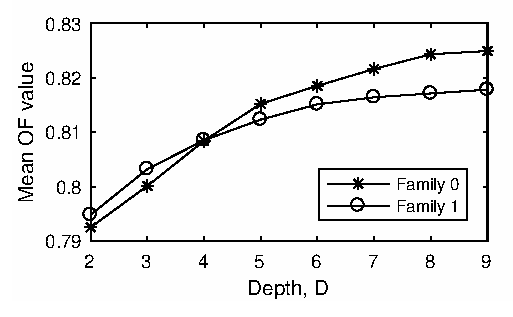
\includegraphics[width=8cm]{chara1.eps}
\caption{\label{fig:manip_to_depth}Minimum value of OF according to depth D for Family 0 and Family 1}
\end{figure}
To match the simulation time-steps, the $\textbf{L}$ set is interpolated through the simulation time. In Figure~\ref{fig:interp}, two different approaches for interpolation are presented, as example for a total simulation time equal to 0.15 s and $D=3$. The first approach (Figure~\ref{fig:interp}a) is similar to a Zero-Order-Hold (ZOH) filter whilst the second (Figure~\ref{fig:interp}b) is a linear interpolation.  In this paper, the linear interpolation is used for simplicity.
\begin{figure}[H]
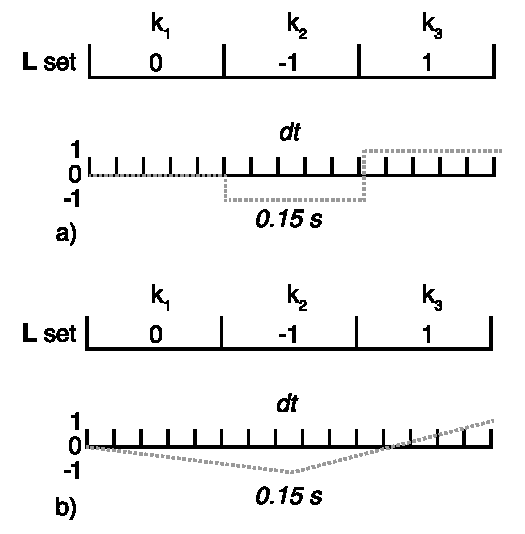
\includegraphics[width=8cm]{chara2.pdf}
\caption{\label{fig:interp}Interpolation approaches. a)ZOH and b)Linear}
\end{figure}
For each gimbal set in a class, the optimization algorithm runs for a set of commanded quaternions in order to obtain the data-set.
The commanded quaternions are converted from Euler angles to quaternions because it is easier to describe and comprehend a manoeuvre as a rotation about roll, pitch and yaw. The manoeuvres given are: independent rotation about roll, pitch, yaw for $\pi$/6, $\pi$/2, 2$\pi$/3, $\pi$ and all the possible permutations of two of those independent rotations.

The structure of the data-set and the histogram of the different $k_i$ values for each element of $\textbf{L}$ set are presented in Figure~\ref{fig:dataset} and Figure~\ref{fig:instances_hist} respectively.
\begin{figure}[H]
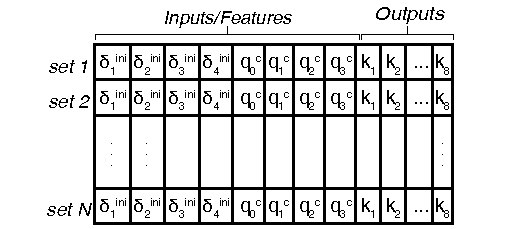
\includegraphics[width=10cm]{chara3.pdf}
\caption{\label{fig:dataset}Data-set structure}
\end{figure}

\begin{figure}[H]
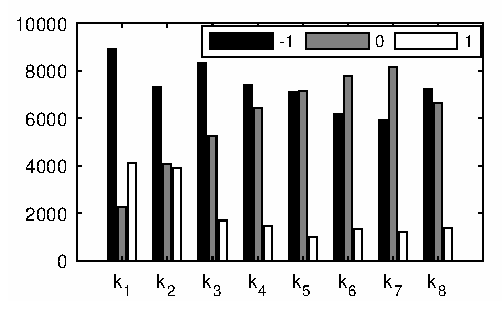
\includegraphics[width=9cm]{chara4.eps}
\caption{\label{fig:instances_hist}Histogram of $k_i$ values}
\end{figure}
It is observed that there is an unequal distribution between the values. The value 1 is observed the least in all elements except for the first. The value -1 is the dominant value for the first four elements and the value 0 is dominant only for the the fifth element.

In a higher capability hardware it would be feasible to use a larger set of commanded quaternions and more than three individual values to describe the motion in the null space. Moreover, including more values in the $\textbf{L}$ set could better match the simulation time-steps improving the interpolation results.

The exact simulation parameters used to produce the data-set are shown in Table~\ref{tab:Parameters}.

\begin{specialtable}[hbt!]
\caption{\label{tab:Parameters} Simulation Parameters}
\begin{tabular}{lcccc}
\toprule
\textbf{Parameter}&\textbf{Value}\\
\midrule
Moment of Inertia \textbf{J}& $\mathrm{diag}([1, 1, 1])$ $\mathrm{kgm^2}$\\
Momentum $h_0$ & 1 Nms  \\
Time-step dt&0.1 s\\
Simulation time& 7 s\\
PID, $K_p$, $K_i$, $K_\omega$ &20, $10^{-5}$, 15\\
Skew angle $\beta$ & 54.73 $ \mathrm{deg}$\\
$\dot{{\delta}}_{th}$ &50 $\mathrm{deg/s}$\\
$k_{max}$ & 0.7\\
D&8\\
\bottomrule
\end{tabular}
\end{specialtable}
 
 
 
 \section{Data Utilization}
The data-set derived does not contain all the possible initial gimbal angles nor all the possible commanded quaternions. Hence, it is important to exploit those data to predict the value of the $\textbf{L}$ set even for these initial gimbal angles and commanded quaternions that are not included in the data-set. To do that, two different ML techniques are utilized.
The input data in both techniques are standardized, i.e the values of each column are individually normalized so that each input data have $\mu=0$ and $\sigma=1$. A training data-set of $N=15300$ %14535
different input samples is used to train the ML systems whilst 765 different samples are used for validation. Without loss of generality, in this paper, only the Family 0 is studied due to hardware limitations and the long time required to derive the data-set for each class. 
\subsection{Deep Neural Network}
The first technique is using eight different DNNs, each one to predict one element of the $\textbf{L}$ set. The algorithm attempts to estimate the mapping function from the input variables to the categorical output variables.
Each DNN has eight (8) neurons in the input layer, four (4) for the commanded quaternion and four (4) for the initial gimbal angles. The  $k_{max}$ value is constant and can be ignored in encoding the different $k_i$ values. Three bits are used for the categorical representations to create the three classes as $-1-> [1,0,0]$, $0->[0,1,0]$ and $1->[0,0,1]$. Thus, the output layer of each DNN consists of three neurons which represent the $k_i$ as described in the previous section. The selection of the optimal DNN architecture is generally problem-dependent and even though trial and error might work, there is no guarantee that it will lead to the optimal solution. Several studies have been done to optimize the topology of such networks, many of them making use of genetic algorithms \cite{DelgadoGA,IdrissiGA,ArifovicGA}. Some thumb rules still exist that roughly determine some good DNN architectures. In \cite{Huang} the number of hidden neurons $N_h$ for the first hidden layer is selected as $N_h=\sqrt{(m+2)N}+2\sqrt{N/(m+2)}$ and for the second hidden layers as $N_h=m\sqrt{N/(m+2)}$ , where $m$ is the number of output neurons and $N$ is the number of sample data. The formula $N_h=(N_{in}+\sqrt{N})/L$ where $L$ is the number of hidden layers and $N_{in}$ is the number of input neurons is also proposed \cite{Ke}. Other methods have also been discussed in \cite{Shibata,Doukim,Yuan}. In this paper, three hidden layers are used with 64 neurons in each one. It has been observed that more neurons and layers, not only increase the ML system complexity requiring a longer training time but also deteriorate the performance because of overfitting. There are 8 neurons in the input layer and 3 neurons in the output layer as described earlier.
A visualization of the $i^{th}$ DNN model predicting the corresponding output $k_i$ is shown in Figure~\ref{fig:DNN_vis}.
\begin{figure}[H]
\includegraphics[width=8.5cm]{DNN_vis.eps}
\caption{\label{fig:DNN_vis}Visualization of the DNN model}
\end{figure}

The activation function of each neuron in the input and hidden layers is the Rectified Linear Unit:

\begin{subnumcases} {\label{fx} f(x)=}
       0, & for $x \leq 0$\\
       x, & for $x > 0$
\end{subnumcases}
The activation function for the neurons in the output layer is the sigmoid function:

\begin{equation}
f(x)=\frac{1}{1+e^{-x}}
\end{equation}
The batch size of the DNN, which denotes the number of data samples that will be propagated through the network before updating the weights of the network, is equal to 64. Selecting the batch size is a trade off among less training time and better training results.
The RMSprop algorithm \cite{rms} is implemented as the optimizer, the learning rate and the discounting factor of which are selected through trial and error in order to achieve the higher possible accuracy without overfitting. The epoch limit is set to 100 because no further improvement in accuracy is observed after this value.
The categorical cross entropy loss function is used for multi-class classification which is given by:

\begin{equation}
CCE = -\sum_{c=1}^{z} y_{i, c} \log \left(\tau_{i, c}\right)
\end{equation}
where $z$ is the number of classes, $y_{i,c}$ is 0 or 1 indicating whether the sample belongs to class $c$ and $\tau_{i,c}$ is the probability for this sample to belong in class c.

The accuracy of each DNN using the validation data is presented in Table~\ref{tab:DNNaccuracies}

\begin{specialtable}[hbt!]
\caption{\label{tab:DNNaccuracies} DNNs - Accuracy}
\begin{tabular}{lc}
\toprule
\textbf{DNN No.}  & \textbf{Value} \%  \\
\midrule
DNN 1 &  80.8 \% \\
DNN 2 &  83.0 \%\\
DNN 3 &  77.5 \%\\
DNN 4 &  77.5 \%\\
DNN 5 &  76.6 \%\\
DNN 6 &  75.8 \%\\
DNN 7 &  74.2 \%\\
DNN 8 &  67.5 \%\\ 
Total     & 28.1 \%\\
\bottomrule
\end{tabular}
\end{specialtable}

It is expected the total accuracy to be lower than the accuracy obtained by each DNN individually because more than one independent values must be predicted correctly. The total accuracy measured by combining all the DNNs is 28.1 \%. Tuning the parameters of the DNNs differently or changing the size of the training and validation data-set does not significantly improve the results. 

The fact that the number of output data of class 1 are fewer than the data of the rest classes for DNN3-DNN8 is partly responsible for the low total accuracy. Even if all DNNs had the accuracy of the first two DNNs, the final accuracy will not be high enough to make the predictions reliable. The total accuracy can be easily conceived as the product of the individual accuracies even though in practice they are not identical.  Thus, to obtain a high performance ML system for predictions, the individual predictions must be higher than the total accuracy and as the depth D increases there is a demand for even higher individual accuracies (Figure~\ref{fig:individual_accuracies}). For example, to obtain a total accuracy of 85 \%  for $D=3$, the individual accuracies required reach up to 94.7 \%.
\begin{figure}[H]
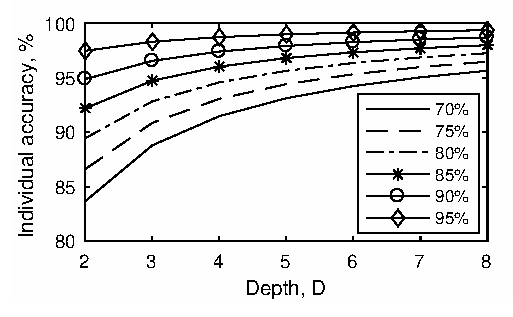
\includegraphics[width=8cm]{chara5.eps}
\caption{\label{fig:individual_accuracies}Individual accuracies according to total accuracy}
\end{figure}

\subsection{Random Forest Classifier}
The second technique used is the RFC. In general, the RFC algorithm generates a large number of individual decision trees that operate as an ensemble. Each individual tree produces a class prediction and the class with the most votes becomes the ML system prediction. Each tree splits from parent to child node following a specific method. They split on the feature and corresponding split point that results in the largest Information Gain (IG) for a given criterion.
Entropy is one of the most frequently used selection criteria for decision trees and it is given by

\begin{equation}
I_{H}=-\sum_{j=1}^{c} \tau_{j}\log _{2}\left(\tau_{j}\right)
\end{equation}
where $\tau_j$ is the proportion of the samples that belongs to class $c$ for a particular node.
The IG can be calculated as 

\begin{equation}
I G\left(D_{\tau}, f\right)=I\left(D_{\tau}\right)-\sum_{j=1}^{m} \frac{N_{j}}{N} I\left(D_{j}\right)
\end{equation}
where $f$ is the feature split on, $D_\tau$ the data-set of the parent node, $D_j$ the data-set of the $j^{th}$ child node, I the impurity criterion, $N$ the total number of samples and $N_j$ the number of samples at $j^{th}$ child node. 200 estimators are used because increasing the number of estimators above this value does not improve the resulting accuracy. All nodes are expanded until all children are pure. The RFC is studied using two approaches. In the first, the RFC is implemented to predict the whole $\textbf{L}$ set at once given the input gimbal and quaternion values. In the second, the RFC predicts each value in L set individually. 
A visualization of the two RFC approaches is shown in Figure~\ref{fig:RFC_vis}.
\begin{figure}[H]
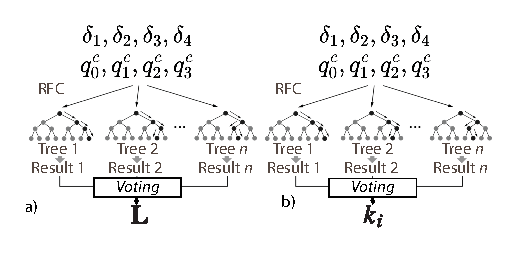
\includegraphics[width=8.5cm]{RFC_vis.eps}
\caption{\label{fig:RFC_vis}Visualization of the RFC, a) 1$^{st}$ and b) 2$^{nd}$ approach}
\end{figure}

The maximum number of inputs the algorithm considers when looking for the best split is selected through trial and error to achieve the best accuracy. For the first approach, it is found to be equal to 7 and the accuracy in the validation data is 75.2 \% with mean absolute error 0.098. Even though not all classes have an equivalent number of samples, the RFC is capable of predicting all three with enhanced accuracy.

In the second approach, each RFC is trained to predict each $k_i$ value individually, the number of estimators remains the same and the maximum number of inputs is set to 3. Regardless of the RFC approach used, the RFC technique always presents a better accuracy compared to this obtained by the DNNs.  
The total accuracy for the second approach is equal to 71.8 \% and the mean squared error 0.109. The accuracies are shown in Table~\ref{tab:RFCaccuracies}.

\begin{specialtable}[hbt!]
\caption{\label{tab:RFCaccuracies} RFC - Accuracies}
\begin{tabular}{lcc}
\toprule
\textbf{RFC No.}  & \textbf{Approach 1} & \textbf{Approach 2}  \\
\midrule
RFC 1 &  94.0 \%  & 92.7 \%   \\
RFC 2 &  93.1 \%  & 92.4 \%   \\
RFC 3 &  91.8 \%  &91.9 \%    \\
RFC 4 &  93.3 \%  & 91.2 \%   \\
RFC 5 &  93.3 \%  &91.2 \%    \\
RFC 6 &  91.2 \%  &90.5 \%    \\
RFC 7 &  91.1 \%  &89.3 \%    \\
RFC 8 &  87.3 \%  &88.1 \%    \\ 
Total   &  75.2 \%  &71.8 \%    \\
\bottomrule
\end{tabular}
\end{specialtable}

\section{Simulation Results}
After defining and training the ML systems, an initial gimbal angle set and a commanded quaternion are selected to predict the null space motion of the system and evaluate the performance of DNNs and RFC. The selected angle set is $\boldsymbol{\delta}^{ini}=[\delta_1^{ini}, \delta_2^{ini}, \delta_3^{ini}, \delta_4^{ini}]^T=[0, 0, 0, 0]^T$ $\text{deg}$ because it is easy to verify that it belongs to family 0.  Without any loss of generality, the commanded manoeuvre is selected to be a rotation about one axis for simplicity, and the value of the commanded quaternion is selected randomly as $\textbf{q}^c=[0.6178,   -0.7863  ,0 ,0]^T$ which corresponds to a -103.69 deg rotation about the roll axis. A 2.7~GHz Inter Core i5 with 8~GB of RAM computer was used and all the simulations were run on the operating system macOS Big Sur in Matlab® R2016b.

For these inputs, the DNNs prediction is $k_{max}[-1,     1,    -1,    0,     0,     0,     0,     0]$. The RFC prediction in the first approach is $k_{max}[1,     1,    -1,    0,     0,     0,     0,     0]$ whilst in the second approach is $k_{max} [-1,     -1,    -1,    0,     0,     0,    0,     0]$. 
All three predictions have in common that the last five elements are zero. This is expected because the low performance configuration is encountered near the beginning of the simulation where the ML systems predict a non zero null space motion. After this state, there is no need for null motion since every gimbal configuration after the singularity corresponds to a better performance index. As a result, the rest of the elements are zero.
The gimbal rates and the manipulability index for each prediction are presented in Figs. \ref{fig:predNSP}-\ref{fig:predRFC2} and the results of the null space projection (NSP) upon the Moore-Penrose pseudo-inverse are also shown for comparison. This NSP steering law is given by

\begin{equation}
\label{eq:NSPeq}
     \dot{\boldsymbol{\delta}}=\textbf{A}^\# \dot{ \textbf{h}}+\kappa_{ns}(\textbf{I}_{4x4}-\textbf{A}^\#\textbf{A})\nabla w(\boldsymbol{\delta})
\end{equation}
where $\kappa_{ns}$ is a constant gain equal to 2, $\textbf{I}_{4x4}$ is the 4 by 4 identity matrix and $\nabla w(\boldsymbol{\delta})$ indicates the gradient of the manipulability index with respect to the gimbal angles.

Similarly to most ML techniques, the derivation of the data-set and the training of the model can be done offline without being involved in the operation of the system. Thus, a total time comparison between the NSP and the ML techniques would be unfair.  In order to measure the execution time difference, i.e the time it takes for all the calculations needed until the end of the simulation, the training and data-set derivation time are excluded. Table~\ref{tab:exectime} shows the percentage difference in the execution time with respect to the NSP. It is observed that there is a 50.9 \%, 51.1 \% and 48.4 \% improvement in the execution time when the ML techniques are utilized compared to the NSP. This is expected because there is no need to calculate the gradient of the performance index of the Equation~(\ref{eq:NSPeq}) which is the most time consuming part. The proposed ML methods offer the advantage of directly executing the null motion through commanding the $\textbf{L}$ set to the CMG cluster. No need of additional computational power is required since the model generation, the training and the predictions of $k_i$ values are executed a priori.

\begin{specialtable}[hbt!]
\caption{\label{tab:exectime} Execution time}
\begin{tabular}{lc}
\toprule
\textbf{ML Model}  &  \textbf{Percentage}   \\
\midrule
DNN &  -50.9 \%       \\
RFC 1 & -51.1 \%    \\
RFC 2 &  -48.4 \%     \\
\bottomrule
\end{tabular}
\end{specialtable}


The gimbal angles and the manipulability index when the NSP is used are shown in Figure~\ref{fig:predNSP}a and Figure~\ref{fig:predNSP}b respectively. At t=1.1 s the gimbal angles are $[ -50,  -1.4,   43.7 ,   5.9]$ $ \text{deg}$ and the minimum value of the manipulability index equals to 0.935 is obtained. In Figure~\ref{fig:predDNN}a and Figure~\ref{fig:predDNN}b the results for the null motion predicted by the DNNs are presented. The minimum value of the index equals to 0.7144 and is observed at t=5.8 s when the gimbal angles configuration is $[-15.2, 15.3, -17.7, 17.1]$ $\text{deg}$. Figure~\ref{fig:predRFC1}a and Figure~\ref{fig:predRFC1}b illustrate the results for the null motion predicted by the first approach of the RFC. Similarly to the NSP, the minimum index value is obtained at t=1.1 s but the configuration at this time is $[-37.5  ,  1.5 ,  50.0 , -11.4]$ $\text{deg}$. This leads to a higher minimum index value, equal to 0.9978. The results for the second approach of the RFC can be seen in Figure~\ref{fig:predRFC2}a and Figure~\ref{fig:predRFC1}b. The minimum index value and the time it is obtained are the same as previously. Although, significantly different gimbal angle profiles are presented that result in higher manipulability maximum. In addition, constantly higher values are obtained after t=3 s compared to the first approach of the RFC.
It is expected that the NSP will present a higher performance index after the low performance configuration because it aims to improve the value of the manipulability index locally. In contrast, the ML techniques are implemented to exclusively maximize the minimum index value across the desired manoeuvre, not the performance index in each time-step. The main drawback of NSP is that it drives the system to higher performance configurations exploring the possible movements in the gimbal space locally. Hence, it is possible to ignore a path in gimbal space that results in a higher minimum index value because the path locally decreases the manipulability index. Such problems are avoided with global steering approaches, as the techniques described in this paper. It is expected the RFC approaches to present a lower manipulability index value after t=1.1 s compared to NSP, when the system has overpass the singularity. In contrast, the prediction made by DNNs results in a lower minimum manipulability value than this obtained by the NSP indicating that the DNNs are unable to make useful predictions for the specific application.
In terms of attitude error, all the manoeuvres are executed with zero attitude error because the null space motion does not affect the attitude of the system. 

\begin{figure}[H]
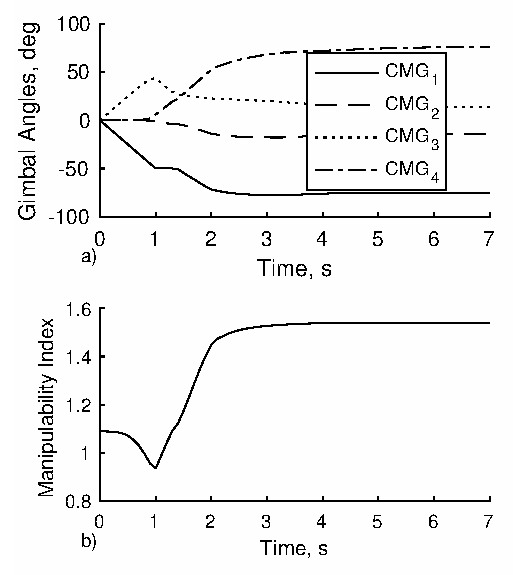
\includegraphics[width=7cm]{chara6.eps}
\caption{\label{fig:predNSP}Simulation results with NSP. a) Gimbal angles, b) Manipulability index}
\end{figure}
\begin{figure}[H]
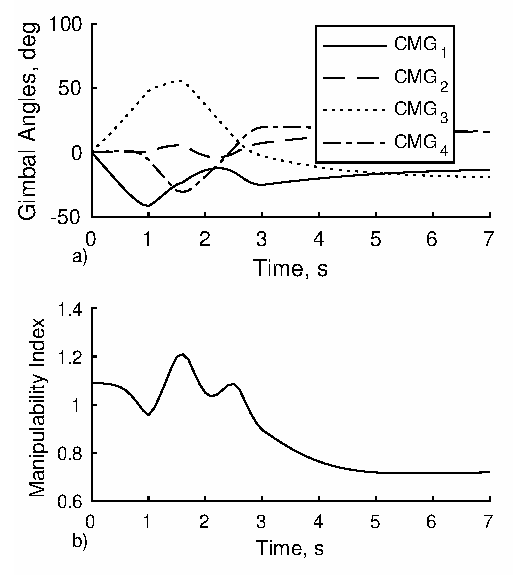
\includegraphics[width=7cm]{chara7.eps}
\caption{\label{fig:predDNN}Simulation results with DNN. a) Gimbal angles, b) Manipulability index}
\end{figure}
\begin{figure}[H]
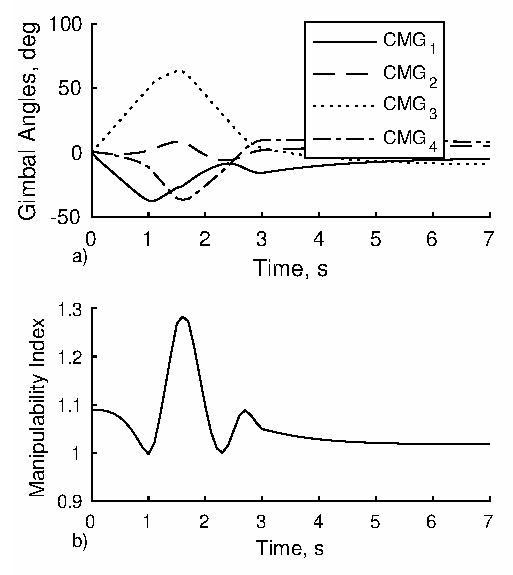
\includegraphics[width=7cm]{chara8.eps}
\caption{\label{fig:predRFC1}Simulation results with RFC - $1^{st}$ approach. a) Gimbal angles, b) Manipulability index}
\end{figure}
\begin{figure}[H]
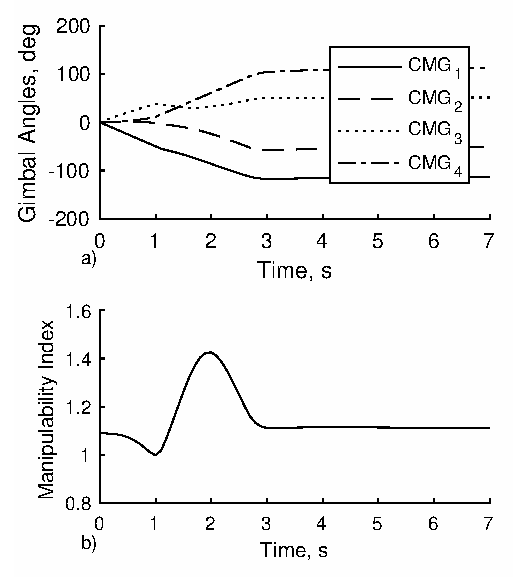
\includegraphics[width=7cm]{chara9.eps}
\caption{\label{fig:predRFC2}Simulation results with RFC - $2^{nd}$ approach. a) Gimbal angles, b) Manipulability index}
\end{figure}
It has been proven that the first approach of the RFC provides a gimbal angle trajectory, in the null space, that results in the highest minimum manipulability value while it has been shown that this RFC model results in the highest accuracy among the examined models. Even though NSP can be implemented on board, it has been shown that when the $\textbf{L}$ set is commanded directly to the satellite, there is a significant improvement in the execution time required, as measured in the simulation. 

The main downside of the proposed ML models is that they are limited by the physical characteristics of the system used to derive the training and the test data. In this paper, the identity matrix is selected as the inertia matrix of the satellite for simplicity, even though it is unrealistic. However, the complexity of the problem remains the same whether the inertia matrix is the identity matrix or a more complex matrix that depicts the characteristics of a satellite in a real-life application scenario. 
Moreover, selecting a higher value of $D$ would allow to decide the null space motion in shorter time intervals even though it would require more time to derive the data-set and train the ML model. Nonetheless, Figure~\ref{fig:manip_to_depth} illustrates that increasing the depth values does not drastically improve the the mean OF value which indicates the existence of a upper bound in the useful depth value.
The various hyper-parameters associated with the ML implementation have to be selected according to the specific data, i.e their number and reliability, because no universal tuning exists to fit every ML problem. The selection of these variables constitutes a research field which is beyond the scope of this paper. 

Despite the limited capabilities of the presented ML systems, due to hardware and time constraints, the described methodology provides high scalability. It is possible to potentially provide a generalized predictive system, by enriching the current data-set with more manoeuvres and different satellite inertias that can be used as data inputs, while allowing the OF to include more terms like the mean value of a manipulabity index and/or the time the gimbal rates exceed a specific threshold.
 
 
 
 
\section{Conclusion}
Two ML techniques for global steering a pyramid-type 4-Control Moment Gyroscope (CMG) cluster have been investigated in this paper. A novel heuristic algorithm has been developed that calculates the optimal null space motion path, that takes into consideration a manipulability-based Objective Function through the whole manoeuvre, given the initial gimbal angles of each CMG and the commanded quaternion. The generated data-set that relates the initial gimbal angles and the commanded quaternion to the null space motion is used to train two ML systems. Among the two Machine Learning (ML) techniques, the Random Forest Classifier (RFC) presents the best performance, predicting with efficient accuracy the desired null space motion even for manoeuvres that are not included in the training set. A task is selected to evaluate the performance of the system following the predicted null motion derived by each ML technique and the results verify the RFC presents a higher minimum manipulability index compared to the Null Space Projection.
Overall, this study is encouraging the determination of a singularity-free manoeuvre that can be known a priory. The proposed methodology can be easily adapted to every satellite as long as its dynamic model is known, otherwise, the same procedure can be followed only for the kinematics model. Moreover, once the data-set is created and the training of the ML system has been completed, the computational demands to predict the output are significantly low, suggesting that the trained system can be potentially used on board to predict the desired $\textbf{L}$ set in real-time. However, the implementation and the needs of such an approach are beyond the scope of this paper and they are reserved for future work. Finally, this paper could be a framework for approaching the CMG cluster singularity problem using ML techniques.
 
 



%%%%%%%%%%%%%%%%%%%%%%%%%%%%%%%%%%%%%%%%%%


%%%%%%%%%%%%%%%%%%%%%%%%%%%%%%%%%%%%%%%%%%
\vspace{6pt} 

%%%%%%%%%%%%%%%%%%%%%%%%%%%%%%%%%%%%%%%%%%
%% optional
%\supplementary{The following are available online at \linksupplementary{s1}, Figure S1: title, Table S1: title, Video S1: title.}

% Only for the journal Methods and Protocols:
% If you wish to submit a video article, please do so with any other supplementary material.
% \supplementary{The following are available at \linksupplementary{s1}, Figure S1: title, Table S1: title, Video S1: title. A supporting video article is available at doi: link.} 

%%%%%%%%%%%%%%%%%%%%%%%%%%%%%%%%%%%%%%%%%%


\funding{This research received no external funding.}

\institutionalreview{Not applicable.}%In this section, please add the Institutional Review Board Statement and approval number for studies involving humans or animals. Please note that the Editorial Office might ask you for further information. Please add ``The study was conducted according to the guidelines of the Declaration of Helsinki, and approved by the Institutional Review Board (or Ethics Committee) of NAME OF INSTITUTE (protocol code XXX and date of approval).'' OR ``Ethical review and approval were waived for this study, due to REASON (please provide a detailed justification).'' OR ``Not applicable'' for studies not involving humans or animals. You might also choose to exclude this statement if the study did not involve humans or animals.}

\informedconsent{Not applicable.}%Any research article describing a study involving humans should contain this statement. Please add ``Informed consent was obtained from all subjects involved in the study.'' OR ``Patient consent was waived due to REASON (please provide a detailed justification).'' OR ``Not applicable'' for studies not involving humans. You might also choose to exclude this statement if the study did not involve humans.

%Written informed consent for publication must be obtained from participating patients who can be identified (including by the patients themselves). Please state ``Written informed consent has been obtained from the patient(s) to publish this paper'' if applicable.}

% \dataavailability{\hl{ }%In this section, please provide details regarding where data supporting reported results can be found, including links to publicly archived datasets analyzed or generated during the study. Please refer to suggested Data Availability Statements in section ``MDPI Research Data Policies'' at \url{https://www.mdpi.com/ethics}. You might choose to exclude this statement if the study did not report any data.} 

\conflictsofinterest{The authors declare no conflict of interest.} 

%% Optional
% \sampleavailability{Samples of the compounds ... are available from the authors.}

%%%%%%%%%%%%%%%%%%%%%%%%%%%%%%%%%%%%%%%%%%
%% Only for journal Encyclopedia
%\entrylink{The Link to this entry published on the encyclopedia platform.}

%%%%%%%%%%%%%%%%%%%%%%%%%%%%%%%%%%%%%%%%%%
% %% Optional
% \abbreviations{The following abbreviations are used in this manuscript:\\

% \noindent 
% \begin{tabular}{@{}ll}
% MDPI & Multidisciplinary Digital Publishing Institute\\
% DOAJ & Directory of open access journals\\
% TLA & Three letter acronym\\
% LD & Linear dichroism
% \end{tabular}}

%%%%%%%%%%%%%%%%%%%%%%%%%%%%%%%%%%%%%%%%%%
%% Optional
% \appendixtitles{no} % Leave argument "no" if all appendix headings stay EMPTY (then no dot is printed after "Appendix A"). If the appendix sections contain a heading then change the argument to "yes".
% \appendixstart
% \appendix
% \section{}
% \subsection{}
% The appendix is an optional section that can contain details and data supplemental to the main text---for example, explanations of experimental details that would disrupt the flow of the main text but nonetheless remain crucial to understanding and reproducing the research shown; figures of replicates for experiments of which representative data are shown in the main text can be added here if brief, or as Supplementary Data. Mathematical proofs of results not central to the paper can be added as an appendix.


% \section{}
% All appendix sections must be cited in the main text. In the appendices, Figures, Tables, etc. should be labeled, starting with ``A''---e.g., Figure A1, Figure A2, etc. 

%%%%%%%%%%%%%%%%%%%%%%%%%%%%%%%%%%%%%%%%%%
\end{paracol}
\reftitle{References}

% Please provide either the correct journal abbreviation (e.g. according to the “List of Title Word Abbreviations” http://www.issn.org/services/online-services/access-to-the-ltwa/) or the full name of the journal.
% Citations and References in Supplementary files are permitted provided that they also appear in the reference list here. 

%=====================================
% References, variant A: external bibliography
%=====================================
\externalbibliography{yes}
\bibliography{mybib}

%=====================================
% References, variant B: internal bibliography
%=====================================
% \begin{thebibliography}{999}
% % Reference 1
% \bibitem[Author1(year)]{ref-journal}
% Author~1, T. The title of the cited article. {\em Journal Abbreviation} {\bf 2008}, {\em 10}, 142--149.
% % Reference 2
% \bibitem[Author2(year)]{ref-book1}
% Author~2, L. The title of the cited contribution. In {\em The Book Title}; Editor1, F., Editor2, A., Eds.; Publishing House: City, Country, 2007; pp. 32--58.
% % Reference 3
% \bibitem[Author3(year)]{ref-book2}
% Author 1, A.; Author 2, B. \textit{Book Title}, 3rd ed.; Publisher: Publisher Location, Country, 2008; pp. 154--196.
% % Reference 4
% \bibitem[Author4(year)]{ref-unpublish}
% Author 1, A.B.; Author 2, C. Title of Unpublished Work. \textit{Abbreviated Journal Name} stage of publication (under review; accepted; in~press).
% % Reference 5
% \bibitem[Author5(year)]{ref-communication}
% Author 1, A.B. (University, City, State, Country); Author 2, C. (Institute, City, State, Country). Personal communication, 2012.
% % Reference 6
% \bibitem[Author6(year)]{ref-proceeding}
% Author 1, A.B.; Author 2, C.D.; Author 3, E.F. Title of Presentation. In Title of the Collected Work (if available), Proceedings of the Name of the Conference, Location of Conference, Country, Date of Conference; Editor 1, Editor 2, Eds. (if available); Publisher: City, Country, Year (if available); Abstract Number (optional), Pagination (optional).
% % Reference 7
% \bibitem[Author7(year)]{ref-thesis}
% Author 1, A.B. Title of Thesis. Level of Thesis, Degree-Granting University, Location of University, Date of Completion.
% % Reference 8
% \bibitem[Author8(year)]{ref-url}
% Title of Site. Available online: URL (accessed on Day Month Year).
% \end{thebibliography}

% If authors have biography, please use the format below
%\section*{Short Biography of Authors}
%\bio
%{\raisebox{-0.35cm}{\includegraphics[width=3.5cm,height=5.3cm,clip,keepaspectratio]{Definitions/author1.pdf}}}
%{\textbf{Firstname Lastname} Biography of first author}
%
%\bio
%{\raisebox{-0.35cm}{\includegraphics[width=3.5cm,height=5.3cm,clip,keepaspectratio]{Definitions/author2.jpg}}}
%{\textbf{Firstname Lastname} Biography of second author}

% The following MDPI journals use author-date citation: Arts, Econometrics, Economies, Genealogy, Humanities, IJFS, JRFM, Laws, Religions, Risks, Social Sciences. For those journals, please follow the formatting guidelines on http://www.mdpi.com/authors/references
% To cite two works by the same author: \citeauthor{ref-journal-1a} (\citeyear{ref-journal-1a}, \citeyear{ref-journal-1b}). This produces: Whittaker (1967, 1975)
% To cite two works by the same author with specific pages: \citeauthor{ref-journal-3a} (\citeyear{ref-journal-3a}, p. 328; \citeyear{ref-journal-3b}, p.475). This produces: Wong (1999, p. 328; 2000, p. 475)

%%%%%%%%%%%%%%%%%%%%%%%%%%%%%%%%%%%%%%%%%%
%% for journal Sci
%\reviewreports{\\
%Reviewer 1 comments and authors’ response\\
%Reviewer 2 comments and authors’ response\\
%Reviewer 3 comments and authors’ response
%}
%%%%%%%%%%%%%%%%%%%%%%%%%%%%%%%%%%%%%%%%%%
\end{document}











